\chapter{Vorgehensweise und Testverfahren}\label{kap3}
Das folgende Kapitel thematisiert, wie während des Projekts vorgegangen wird, welche Entwicklungsmodelle zum Einsatz kommen und welche Testkonzepte angewendet werden.

\section{Entwicklungsmodell}
Sowohl für die Entwicklung eines Softwaresystems als auch für die Entwicklung von Elektronik haben sich Modelle etabliert, die eine Systematik in den Entwicklungsprozess bringen. Dadurch soll eine hohe Qualität des Entwicklungsprodukts sichergestellt werden. 
Unter Qualität, insbesondere bei Softwaresystemen, werden nach \cite{BasSof} bzw. ISO-Norm 25010 \cite{ISO_25010} Eigenschaften verstanden wie Funktionalität, Zuverlässigkeit, Benutzbarkeit, Effizienz und Änderbarkeit.\\
Für die vorliegende Aufgabenstellung ist ein Softwaresystem zur
\begin{itemize}
	\item Verarbeitung der Sensorik,
	\item Anwendung des Regelgesetzes,
	\item Ansteuerung der Aktorik,
	\item nichtflüchtige Kalibrierung und
	\item selbstständige Fehlererkennung
\end{itemize}
notwendig. Gleichermaßen muss jedoch eine Elektronik entwickelt werden, auf welcher das Softwaresystem ausgeführt wird und durch welche die Schnittstellen zu notwendigen Komponenten hergestellt werden. Um beide Systeme parallel zu entwickeln, wird das V-Modell gewählt, das in \autoref{fig_v_modell} dargestellt ist. 



\subsection{Das V-Modell}

\begin{figure}[H]%
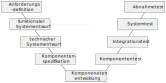
\includegraphics[width=\columnwidth]{./Bilder/fig_v_modell}%
\caption{V-Modell nach \cite{Boehm79}}%
\label{fig_v_modell}%
\end{figure}

Das V-Modell ist ein Vorgehensmodell, dass in verschiedenen Ausführungen existiert. Das hier vorgestellte und angewendete Modell entspricht dem Modell nach \cite{Boehm79}. Als weitere Quelle wird \cite{BasSof} herangezogen und im Folgenden referenziert.
Der linke Zweig stellt dabei die konstruktive Entwicklung dar, während jede Aktivität eine dazu korrespondierende Testaktivität im rechten Zweig besitzt. \\

\subsubsection{Konstruktive Entwicklung (linker Zweig)}
Zunächst wird demnach eine Anforderungsliste im Zuge der \textit{Anforderungsdefinition} erstellt, die die Entwicklungsaufgabe genauer spezifiziert und später eine Überprüfungsgrundlage bietet inwiefern das fertige Gesamtsystem des Wunschsystems entspricht. Daran anschließend wird ein \textit{funktionaler Systementwurf} durchgeführt. Hierbei werden die Anforderungen in Funktionen überführt, die das Gesamtsystem erfüllen muss, um den Anforderungen gerecht zu werden. Darauf folgend findet der \textit{technische Systementwurf} statt. Dafür wird das System in unabhängige Teilsysteme unterteilt und Schnittstellen zur Umwelt ermittelt. Daran logisch anknüpfend wird die \textit{Komponentenspezifikation} durchgeführt. Dafür wird für jede Komponente (elementares Teilsystem) die Aufgabe, das gewünschte Verhalten und Schnittstellen zu anderen Teilsystemen definiert. \\
Den letzten reinen Entwicklungsschritt bildet die \textit{Komponentenentwicklung}. Dabei werden schließlich die einzelnen Komponenten nach der zuvor erarbeiten Spezifikation entwickelt. Eine Komponente stellt dabei ein Teilsystem dar, das eine feste Funktion erfüllt, und in der Regel aus einem Softwareteil und einem Hardwareteil besteht. Beide Teile werden parallel in genauer Abstimmung entwickelt, da die gewünschte Funktion nur durch beide Systeme im Zusammenspiel erfüllt werden kann. Das Softwaresystem besteht dabei in der Regel aus einem Treiber, der die komplexe Hardwareschnittstelle für das Restsystem versteckt und komfortable Schnittstellen bereitstellt. Ein Beispiel dafür stellt der Treiber für den Tauchspulenaktor dar, der eine Pulsweite in Prozent und ein Aktivierungssignal entgegen nimmt. Intern werden dann daraus Steuersignale für die Halbbrücken generiert und über die Elektronikschaltung dem Aktor zugeführt.
Neben Elektronikschaltungen mit zugehörigem Treiber existieren auch \textit{reine Softwarekomponenten}, die unabhängig der Elektronik entwickelt werden wie bspw. eine Verhaltenslogik für ein- und ausgehende CAN-Nachrichten. Ebenso existieren \textit{reine Elektronikkomponenten}, die keinen direkten Bezug zur Software aufweisen und daher unabhängig von dieser entwickelt werden können.\\

\subsubsection{Testaktivitäten (rechter Zweig)}
Alle folgenden Informationen sowie detaillierte Ausführungen bezüglich des Testverfahrens können \cite{BasSof} entnommen werden.\\
Nachdem die Entwicklung aller Komponenten abgeschlossen ist, müssen die einzelnen Komponenten auf die geforderte Funktionalität überprüft werden. Dazu wird jede Komponente so isoliert wie möglich vom Restsystem getestet, ggf. unter Einsatz sogenannter Testtreiber und Platzhalter, um die zu testenden Komponenten mit Testdaten oder Testfällen auszuführen. Durch die Isolation wird sichergestellt, dass die einzelne Komponente als solche funktioniert und Fehlerzustände leichter eingegrenzt und lokalisiert werden können. Jeder Testfall enthält dabei feste Vorbedingungen, Eingabewerte und ein gefordertes Sollverhalten bzw. geforderte Ausgabewerte. Die Auswahl der Testfälle wird durch die Art der Komponenten unterschieden. \textit{Treiber mit zugehöriger Hardwarekomponente} bieten Schnittstellen, die beliebige Zahlenwerte und Kombinationen entgegen nehmen. Daraus resultiert eine quasi unendliche Menge an möglichen Testfällen, die nicht praktikabel getestet werden können. Vollständiges Testen ist daher nicht möglich. Aus diesem Grund werden die Testfälle aus einem Klassifikationsbaum mit anschließender Grenzwertanalyse gewonnen. Dabei wird jeweils mindestens ein Testwert aus jeder Gruppe ausgewählt. Die Gruppierung wird so vorgenommen, dass von jeder Gruppe aus Testwerten gleiches Verhalten angenommen wird. Als Beispiel kann wieder die Ansteuerung des Tauchspulenaktors herangezogen werden. Es wird davon ausgegangen, dass alle Werte zwischen -100 und 0 eine Bewegung in eine feste Richtung bewirken. Dagegen bewirken Werte von 0 bis 100 eine Bewegung in die Gegenrichtung. Werte außerhalb des Zahlenbereichs werden auf entsprechend -100 oder +100 abgerundet. Durch eine Grenzwertanalyse werden diese Gruppen (auch Äquivalenzklassen genannt) noch in Untergruppen unterteilt, in denen die oft kritischen Grenzwerte (-100, 0 und 100) noch eigene Gruppen bilden. Eine Sonderstellung besitzt die Null, weil hier keine Reaktion erwartet wird. Durch kombinatorische Paarbildungen werden darüber hinaus auch beliebige Kombinationen aus abhängigen Eingangswerten, bspw. Aktivierungssignal (enable) und Pulsbreite (PWM in \%), berücksichtigt. Um die Testfallgenerierung durch Klassifikationsbäume zu verdeutlichen, ist in \autoref{fig_klass} der Klassifikatiosbaum grafisch dargestellt. Die untere Zeile aus konkreten Werten stellt beispielhafte Testwerte aus der darüberliegenden Äquivalenzklasse dar. Darunter ist über die Gitterstruktur angedeutet, wie aus der paarweisen Kombination der einzelnen Testwerte Testfälle bestimmt werden. \textit{Testfall 1} entspricht dem Aufrufen des Treibers mit einer PWM von \SI{-100}{\%} und einem aktivierten \textit{enable}-Signal. Es wird daher erwartet, dass der Aktor voll in die negativ definierte Bewegungsrichtung bestromt bzw. beschleunigt wird. Ob die Elektronik als solche den Erwartungen bzw. der Spezifikation entspricht, kann durch Strom-/Spannungs- sowie Temperaturmessungen verifiziert werden. 
\begin{figure}[H]%
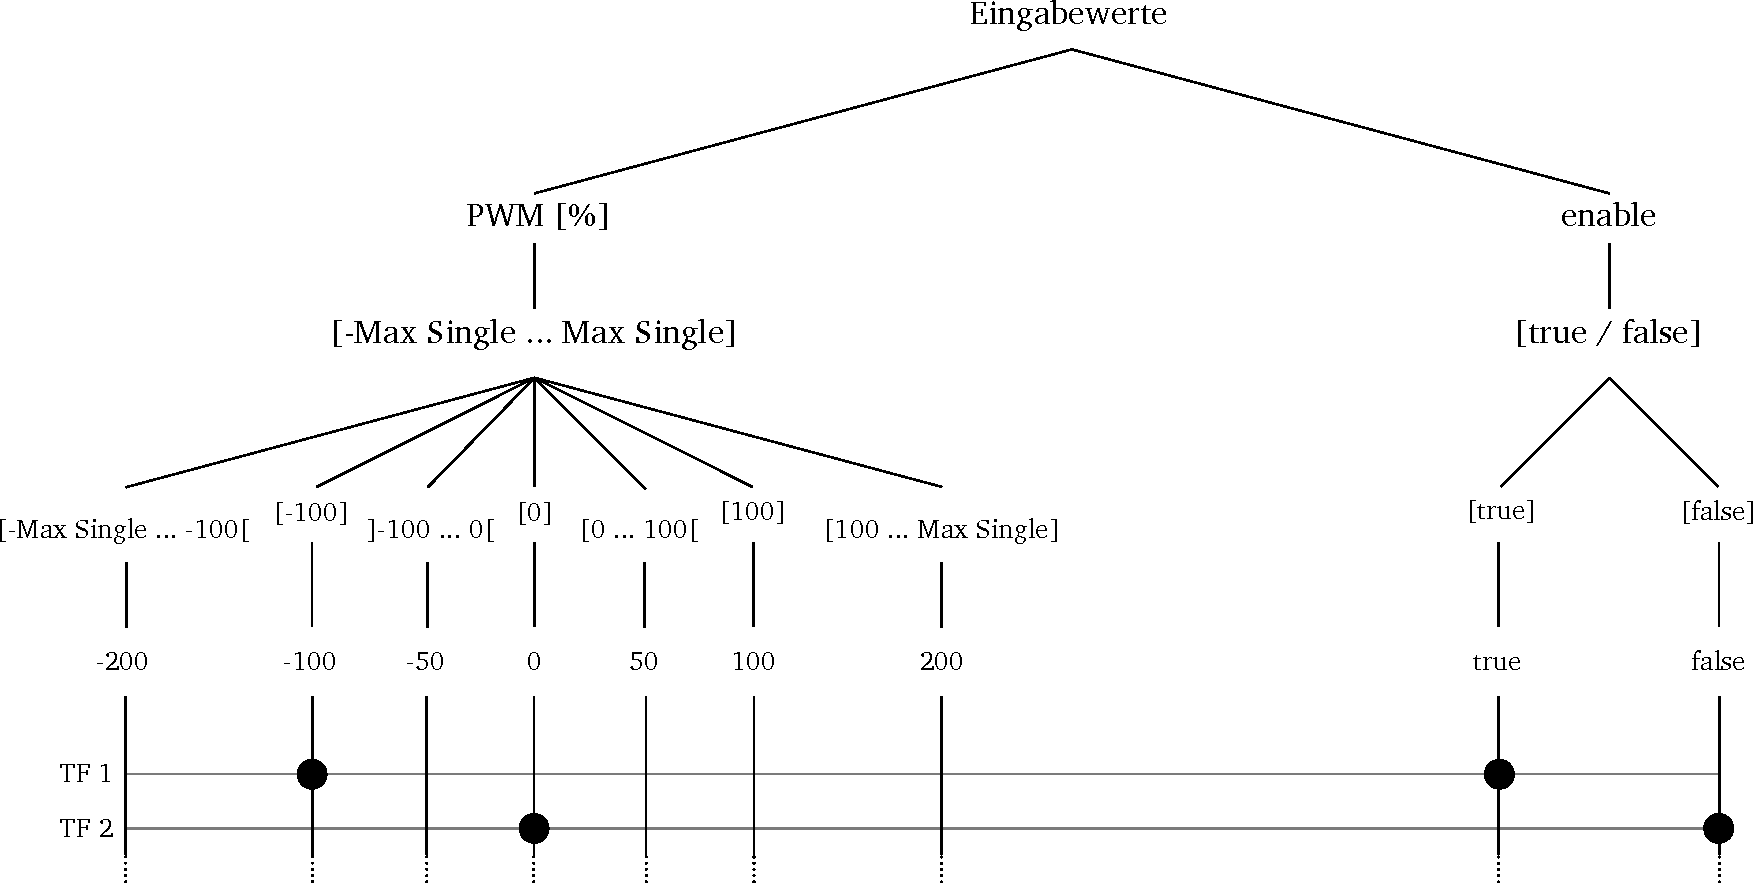
\includegraphics[width=\columnwidth]{./Bilder/fig_klass}%
\caption{Klassifikationsbaum am Beispiel des Motortreibers}%
\label{fig_klass}%
\end{figure}\noindent
Für \textit{reine Softwarekomponenten} hingegen werden Testfälle auf eine geeignetere Weise generiert. Bei Softwarekomponenten auf Basis eines Zustandsautomaten werden Testfälle aus einer zustandsbasierten Testfallgenerierung gewonnen. Dabei wird als Testziel vorausgesetzt, dass alle Entscheidungen (Kanten) eines Zustandsautomaten mindestens einmal ausgeführt werden, was als Entscheidungsüberdeckungskriterium bezeichnet wird. Dieses Kriterium schließt auch automatisch ein, dass alle Zustände (Knoten) besucht worden sind. Wie viele Testfälle getestet werden müssen hängt dabei stark von der Größe und Komplexität des Zustandsautomaten ab.\\
Nach dem Test der einzelnen Komponenten wird eine Integration vollzogen. Unter Integration wird dabei das Zusammenführen der Komponenten zu einem Gesamtsystem verstanden. Es stehen viele Varianten zur Verfügung, dazu zählen \textit{Bottom Up}-, \textit{Top Down}- und \textit{Big Bang}-Integration. Letztere Variante sieht vor, dass alle Komponenten in einem Zug ins Gesamtsystem integriert werden. Auftretende Fehler können jedoch in diesem Fall nur schwierig zugeordnet werden. Günstiger ist daher die \textit{Bottom Up}-Integration, wobei nach und nach Komponenten hinzugefügt werden und übergeordnete Komponenten, die mit mehreren Einzelkomponenten Schnittstellen haben, später integriert werden. Da im vorangehenden \textit{Komponententest} bereits die Komponenten getestet sind, ist im anschließenden \textit{Integrationstest} mit Fehlern zu rechnen, die durch Schnittstellen zwischen den Komponenten hervorgerufen werden. Es kann davon ausgegangen werden, dass die Komponenten intern funktionieren und ausschließlich das Zusammenspiel der Komponenten fehlerhaft ist. \\
Zuletzt entsteht somit ein Gesamtsystem, das darauf getestet werden muss, ob die im \textit{funktionalen Systementwurf} festgelegten Funktionen erfüllt werden. Um dies zu testen werden \textit{Use-Case}-Szenarios erstellt, die eine übliche Nutzung simulieren. Dabei wird von mehreren Akteuren ausgegangen, die mit dem System in der realen Anwendung agieren werden. Der Schaltaktor wird bspw. über ein übergeordnetes Steuergerät (\textit{electrical Control Unit}) angesteuert. Die Schnittstelle wird durch CAN realisiert, sodass ein entsprechendes Steuergerät über CAN Signale/Befehle einen Schaltvorgang anfordern oder eine Fehlermeldung auslesen kann. Einen typischen \textit{Use-Case} würde bspw. ein Schaltbefehl vom neutralen in den zweiten Gang darstellen. Dieser kann erfolgreich ablaufen oder durch eine mechanische Blockade verhindert werden. Abschließend erfolgt der Abnahmetest, der in der Regel durch den Auftraggeber durchgeführt wird. Hier wird explizit verglichen, ob die versprochenen Leistungen im Pflichtenheft auch erreicht werden.\\
Diese und weitere Informationen für den interessierten Leser finden sich in \cite{BasSof}.

\subsection{Konkretes Vorgehen mit inkrementellem Entwicklungsansatz}

Neben dem V-Modell fließen auch inkrementelle Ansätze in die Entwicklung ein. So wird das V-Modell mehrmals durchlaufen, während nach jeder Iteration ein ausführbares und testbares Entwicklungsprodukt vorliegt. Diese Zwischenprodukte entsprechen der Anforderungsliste unter Umständen nur teilweise, sodass mehrere Iterationen bis zu einem zufriedenstellenden Produkt notwendig sind.\\
Für das vorliegende Projekt wird in der ersten Iteration ein Prototyp angestrebt, der bereits die Grundfunktionalitäten bereitstellt. Dies umfasst die Möglichkeit, einen Schaltvorgang nach Anforderungsspezifikation durchzuführen. Dafür muss unter anderem die Aktorik ansteuerbar sein und die Sensorik notwendige und hinreichend genaue Regelgrößen liefern. 
Während der Phase des frühen Prototypings wird der Mikrocontroller auf einem Entwicklungsboard verwendet, um Daten über eine serielle Schnittstelle mit dem PC austauschen zu können. Zusätzlich erfolgt über das Entwicklungsboard die Programmierung des Mikrocontrollers während alle Pins leicht über Stiftleisten erreichbar sind. Die Funktionalität der geplanten Brückenschaltung zur Aktorsteuerung wird dafür zunächst unabhängig vom Aktor getestet. Dies wird der Einfachheit halber auf Steckbrettbasis und durch Anschluss zweier LEDs anstelle des Aktors durchgeführt. So kann sichergestellt werden, dass die Ansteuerung der H-Brücke durch den Softwaretreiber den Erwartungen entspricht. Anschließend wird die getestete H-Brückenschaltung auf eine Lochrasterplatine gelötet, da diese den Anforderungen an Strombelastbarkeit des realen Aktors genügt. Somit können neben der Funktionalität auch weitere Aspekte wie Temperaturentwicklung und Einfluss der \textit{slew rate} geprüft werden.
Die Elektronik zum Auslesen des Lagesensors, welcher bereits von Vorgängerprojekten genutzt wurde, wird ebenfalls auf einem Steckbrett realisiert. Dabei werden verschiedene Ansätze in Soft- und Hardware verfolgt um den Einfluss auf die Genauigkeit der Lagemessung zu prüfen.
Nachdem Lagesensorik und Aktoransteuerung erfolgreich getestet sind, kann die Regelung des Aktors durch eine frühe Version des Hauptprogramms getestet werden. Die CAN-Schnittstelle wird dabei noch durch eine serielle Schnittstelle zum PC ersetzt. Bei diesem ersten Prototypen werden Anforderungen an Größe, Effizienz oder Integrierbarkeit nicht verfolgt. Der Protoyp hat gezeigt, dass prinzipiell eine Regelung durch die entwickelten Komponenten möglich ist, allerdings der Schaltvorgang in Neutral noch starkes Überschwingen ausweist. Diese Erkenntnisse werden in den nächsten Iterationen berücksichtigt. 
Bei folgenden Iteration wird versucht über geeignete Maßnahmen (bspw. durch eine angepasste Komponentenspezifikation) bisherige Ergebnisse zu verbessern und weitere Anforderungen zu erfüllen. 
Hierfür rückt besonders die iterative Weiterentwicklung der Software in den Vordergrund, während Hardwarekomponenten wie Temperatur-, Strom- und Spannungssensorik in den Prototypen eingepflegt werden. Eine nichtflüchtige Kalibrierung wird in das Softwaresystem eingearbeitet und anhand künstlicher Spannungsunterbrechungen getestet. Weiterhin wird die CAN-Schnittstelle eingeführt und für unterschiedliche Sendegeschwindigkeiten und Kabellängen getestet.\\
Einen wesentlichen Iterationsschritt stellt schließlich der Übergang von Steckbrett- auf Platinenbasis dar. Durch diesen Übergang treten weitere Anforderungen wie Baugröße und Integrierbarkeit in den Vordergrund. Nach dem letzten Iterationsschritt sollten alle Anforderungen nachweislich erfüllt sein, sodass ein erfolgreicher System- und Abnahmetest durchgeführt werden kann. In \autoref{fig_entw_evo} sind die Iterationen symbolisch dargestellt.

\begin{figure}[H]%
\centering
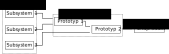
\includegraphics[width=0.8\columnwidth]{./Bilder/fig_entw_evo4}%
\caption{Bildliche Darstellung des Prototypings (Iterationsprozesses)}%
\label{fig_entw_evo}%
\end{figure}
